\documentclass[12pt,a4paper]{scrbook}
\usepackage[utf8]{inputenc}
\usepackage[ngerman]{babel}
\usepackage{graphicx}
\usepackage{geometry}
\geometry{left=2.00cm, right=2.00cm, top=2.00cm, bottom=2.00cm}
\pagestyle{empty}

\newcommand{\Kap}[2][keinS]{%
	\def\varX{S}%
	\def\varY{#1}%
	\if\varX\varY%
	Kapitel~\ref{#2},~Seite~\pageref{#2}%
	\else%
	Kapitel~\ref{#2}
	\fi
}

\begin{document}
\chapter{Testkapitel}
\section{Testabschnitt}
\subsection{Testunterabschnitt}
\clearpage

... siehe \Kap{sec:houses}.

... siehe \Kap[S]{sec:houses}.

\clearpage
\begin{figure}[htb]
	\centering
	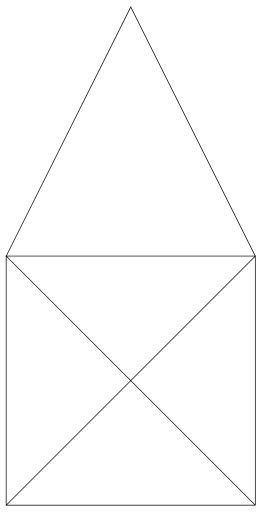
\includegraphics[width=2cm]{house/house.png}
	\caption{Das Haus}
	\label{fig:house}
\end{figure}
\label{sec:houses}
\end{document}